\section{Gravitational waves}
``Space-time tells mass how to move; mass tells space-time how to curve" provides a sufficient summarization of Einstein's theory of general relativity ~\cite{Misner1973}. Insights on high energy astrophyical phenomena (highly massive binary coalescences, spherically assymetric compact objects, etc.) are built into this theory; one being space-time distortions known as gravitational waves. Explicitly, this is shown as a perturbation in the metric tensor defining a local space-time geometry:
\\
\textcolor{red}{Metric tensor}
\\
Such a perturbation arises from a time varying quadrupole moment.
\\
\textcolor{red}{Refer to GR notes}
\\
Information on the progenitors of these systems are encoded in these waves and the detection and study of them open an entirely new chapter in astronomy.
\subsection{Gravitational wave astronomy}
Gravitational wave detection has a history starting with a desire for further experimentation in gravity. The literature provided by those part of this history offers important motivations and details of the field supplemented by fascinating and humbling stories.

As of September 14th 2015 the LIGO detectors transitioned from the most sensitive differential displacement sensors ever built to also becoming the first ever gravitational wave observatory with ?? confirmed gravitational wave detections from O1 to O3b as of the date of the submission of this dissertation. 
\textcolor{red}{Figure of detections published from O1 to the end of O3.}
\newpage
\section{Detector configurations}
\subsection{Interferometry with a Michelson configuration}
Initially used by Michelson and Morley for an experiment intended to support the existence luminiferous aether, the optical design was discovered nearly a century later to lend itself to a gravitational wave detection schema. The perpendicular beam paths set by the beamsplitter and two end mirror offer create an interference condition of the returning beams at the beamsplitter; which is disrupted by differential path length changes between the beam paths which can be tracked at the (anti-symmetric) detection port using the following equation:

\begin{equation}
	P_\mathrm{out} = \frac{P_\mathrm{in}}{2}(1+\mathrm{cos}( 4\pi/\lambda (L_x - L_y))
\end{equation}

Knowing the Michelson will register a diffential arm shift with adjusting fringe brightness, the length response can be reframed into a phase response of the Michelson from a time-dependent metric perturbation:

\begin{equation}
\Delta \phi(t) = \phi_x(t) - \phi_y(t) =  \int_{t-2L/c}^{t} \Omega \bigg[1 + \frac{1}{2}h(t)\bigg]dt - \int_{t-2L/c}^{t} \Omega \bigg[1 - \frac{1}{2}h(t)\bigg]dt 
\end{equation}

\begin{equation}
\Delta \phi (\omega) = h_0\frac{2 L \Omega}{c}e^{-i L \omega / c} \frac{\mathrm{sin}(L \omega /c)}{L \omega /c}
\end{equation}

Where $h(t)$ is the time dependent metric perturbation from a gravitational wave with amplitude $h_0$ angular frequency $\omega$, L is the length of the interferometer arms, c is the speed of light, $\Omega$ is the angular frequency of light.


\begin{figure*}[h!]
	\begin{subfigure}{\includegraphics[width=.45\textwidth,page=2]{INTRO/ifo_configs.pdf}}
  	\end{subfigure}
  	\hfill
  	\begin{subfigure}{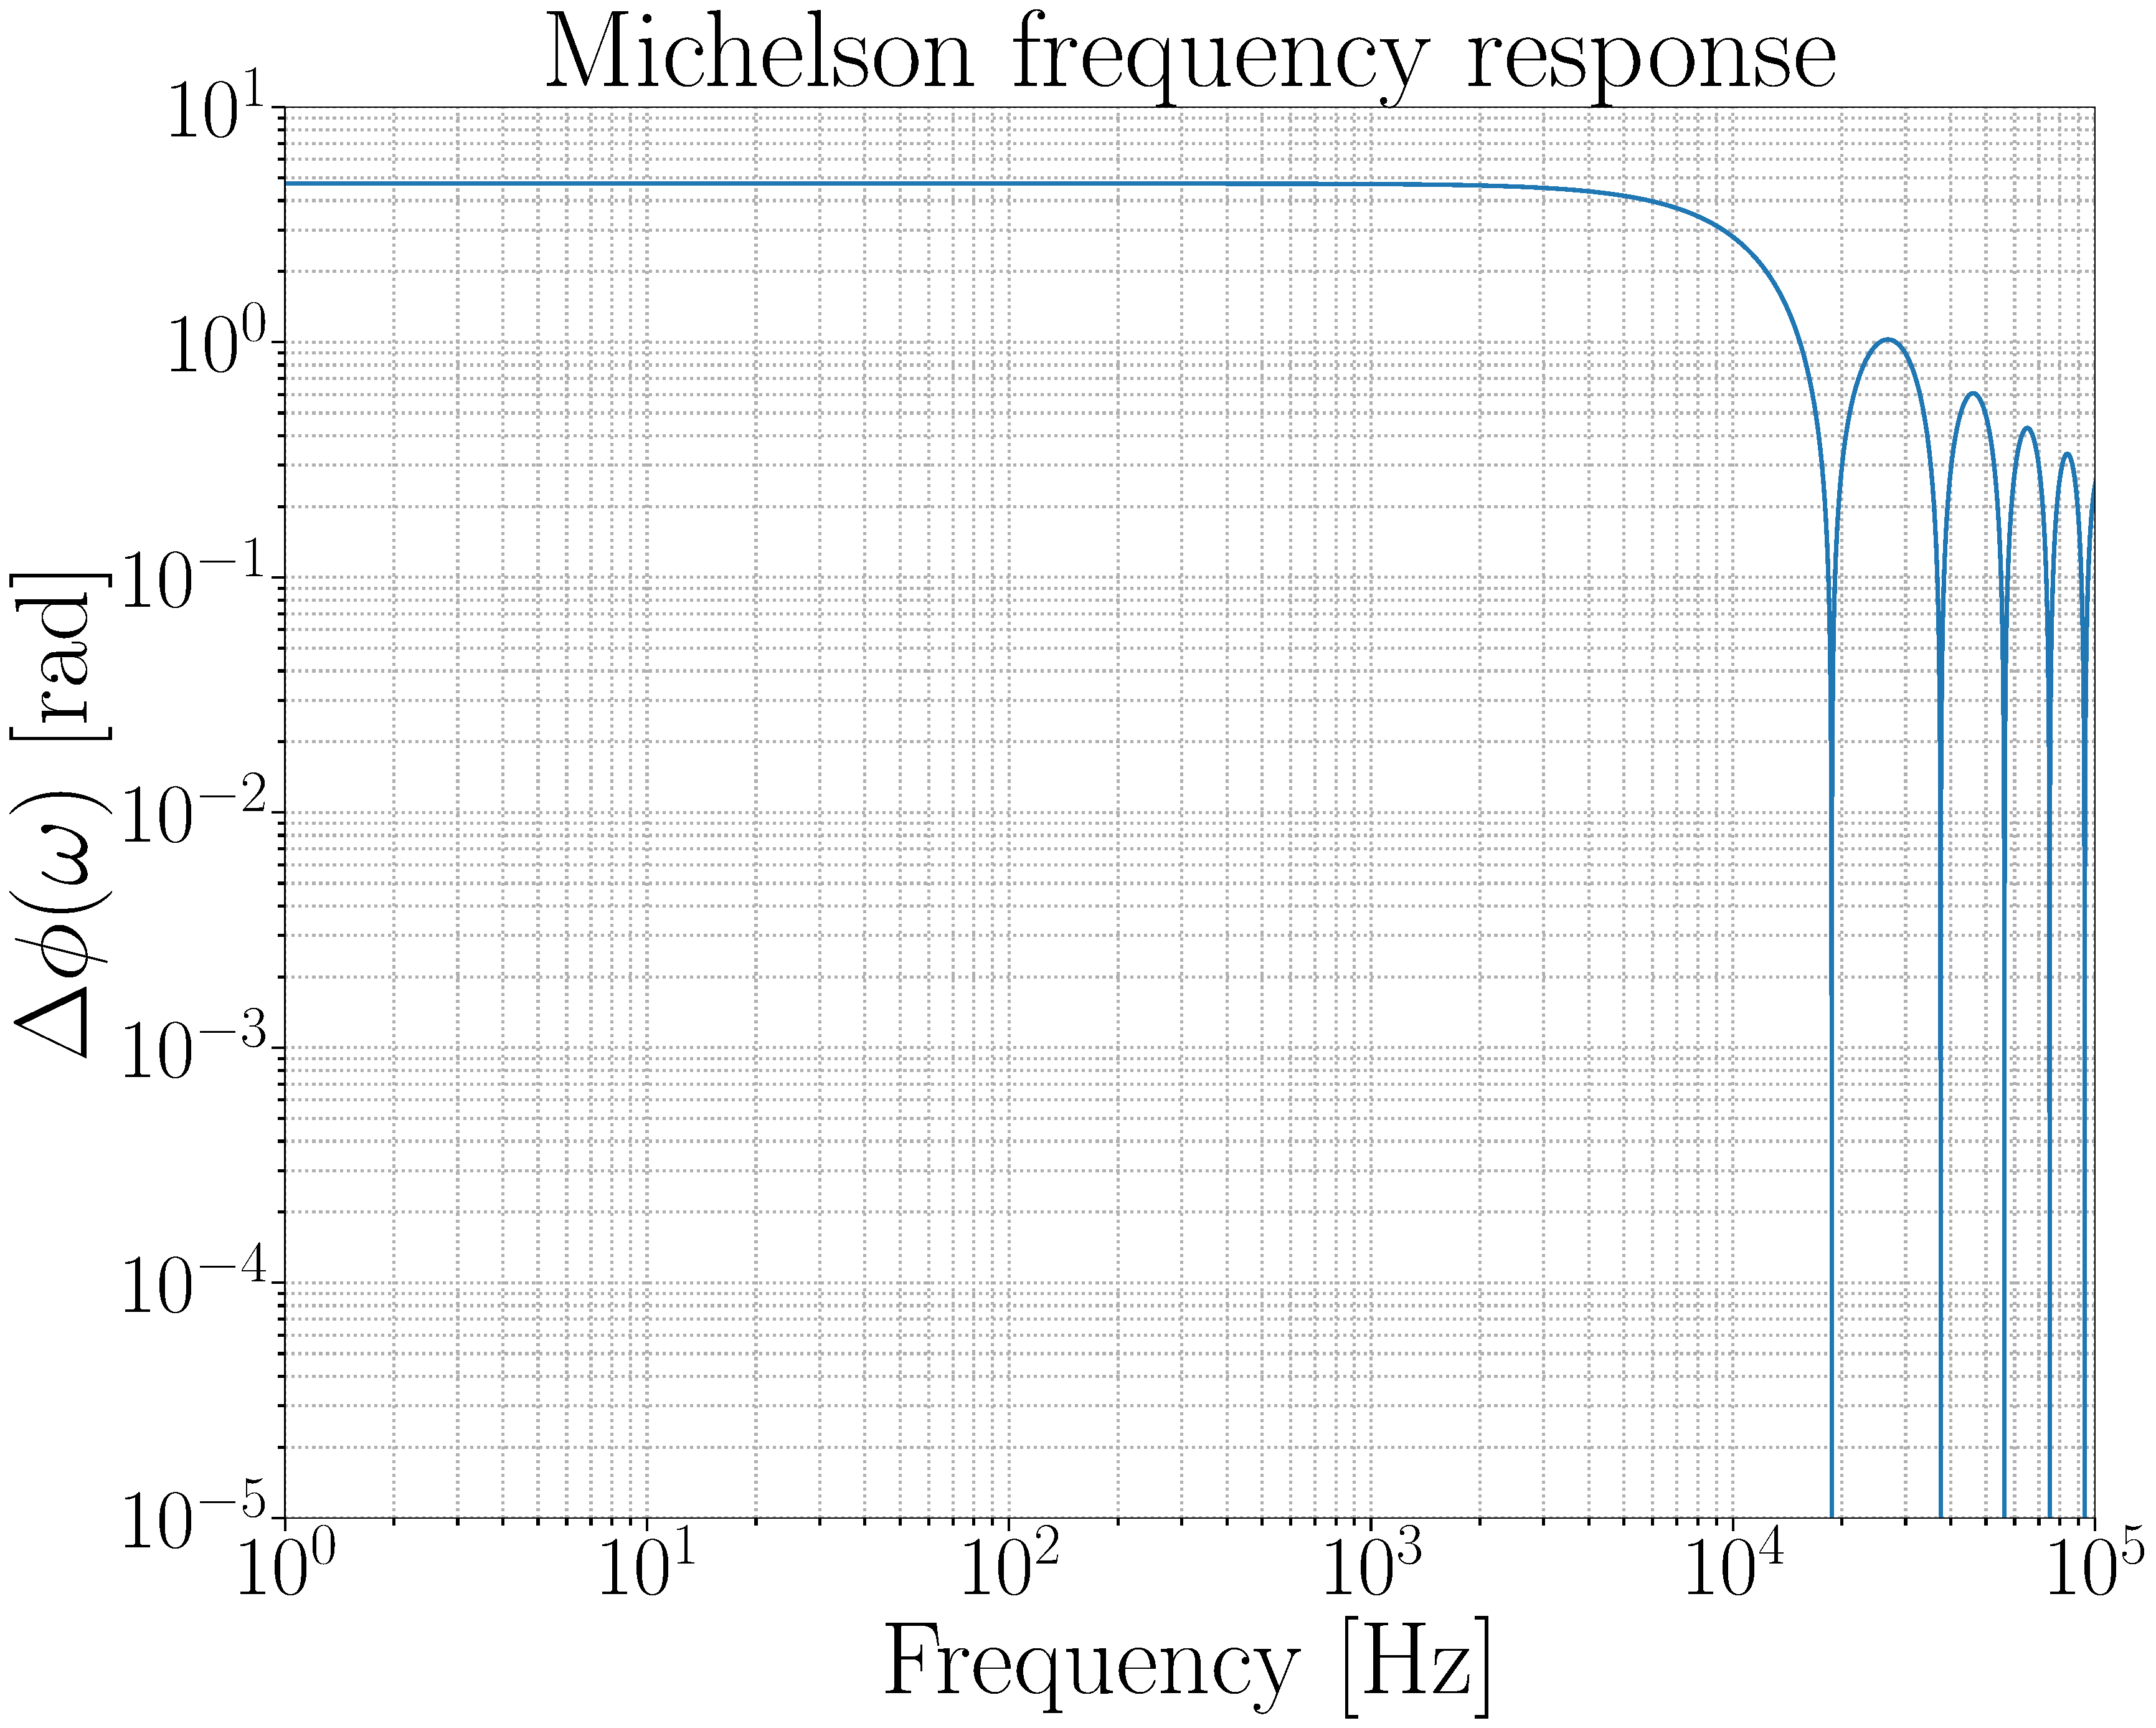
\includegraphics[width=.5\textwidth]{figs/mich_fr.pdf}}
 	 \end{subfigure}
  	\hfill
  	\caption{\textcolor{red}{PENDING UPDATE} The simple 4km Michelson with associated differential arm length response (left is optical schema, right is frequency response)}
  	\label{fig:mich}
\end{figure*}
\FloatBarrier

Assuming a LIGO configuration (with 4km arm length), the differential arm response provides a reasonable optical gain proportional to the differential phase until you reach a frequency that coorelates to a integer number of gravitational wave half periods $\mathrm{n}\lambda_gw / 2$ to the interferometer arm length in such a way that the response is null.

\subsection{Fabry-P\'{e}rot Michelson (FPMI)}
At the time of proposal, financial and physical constraints for terrestrial gravitational wave detectors required a compact solution for extending arm lengths on the build~\cite{}. Two proposed techniques were considered: the Delay Line and the Fabry-Perot cavity. Though choice ultimately became the Fabry-Perot cavity.


\subsubsection{The Fabry-P\'{e}rot cavity}
Prior to this discussion, the Michelson interferometer would not provide a sufficient optical gain for any practical arm length, so how does a Fabry-P\'{e}rot cavity offer a solution or even relate?  To understand we consider an an idealized coherent light wave encountering an optical cavity with input and output mirror transmission and reflection coefficients of $t_1$, $r_1$ and $t_2$, $r_2$ respectively (and assuming a loss coefficient of $l=0$).

\textcolor{red}{Figure of Fabry-P\'{e}rot cavity}

It enters the cavity only after passing the input mirror with a field amplitude reduced by the mirror reflection coefficient. So far this doesn't seem quite useful as we have already reduced the power for the phasefront of interest, until the realization that said phasefront will stay stored within the cavity until its final photon exits the cavity; this ``cavity storage time" ($\tau_s \appropto L r_1r_2$) can be imagined as length elongation with the phasefront travel history encoded in the arrival time of the phasefront's photons back at the light source source. But this assumes that the photons of belonging to a particular phasefront can be experimentally tracked, and with a constant source at the cavity input the phasefronts entering the cavity are superimposed onto the circulating cavity field and, more often than not, add incoherently which can makes this thought experiment this seem silly. It is with careful microscopic tuning of mirror positions that there can be coherent addition of these intra-cavity phasefronts and the true novelty of the Fabry-P\'{e}rot can be fully realized. This condition described is known as cavity resonance and appears when deriving the cavity reflection and transmission coefficients:

\begin{equation}
	r_c = -r_1 + \frac{t^2_1r_2 e^{-i2kL}}{1-r_1 r_2 e^{-i2kl}}
\end{equation}

\begin{equation}
	t_c = \frac{t_1 t_2 e^{-ikL}}{1-r_1 r_2 e^{-i2kL}}	
\end{equation}


The storage time of the phasefronts within the cavity can now be correlated to the amplitude of the superimposed intracavity field, which can be measured as a power reflected and/or transmitted from the resonant cavity. 

\begin{figure}[H]
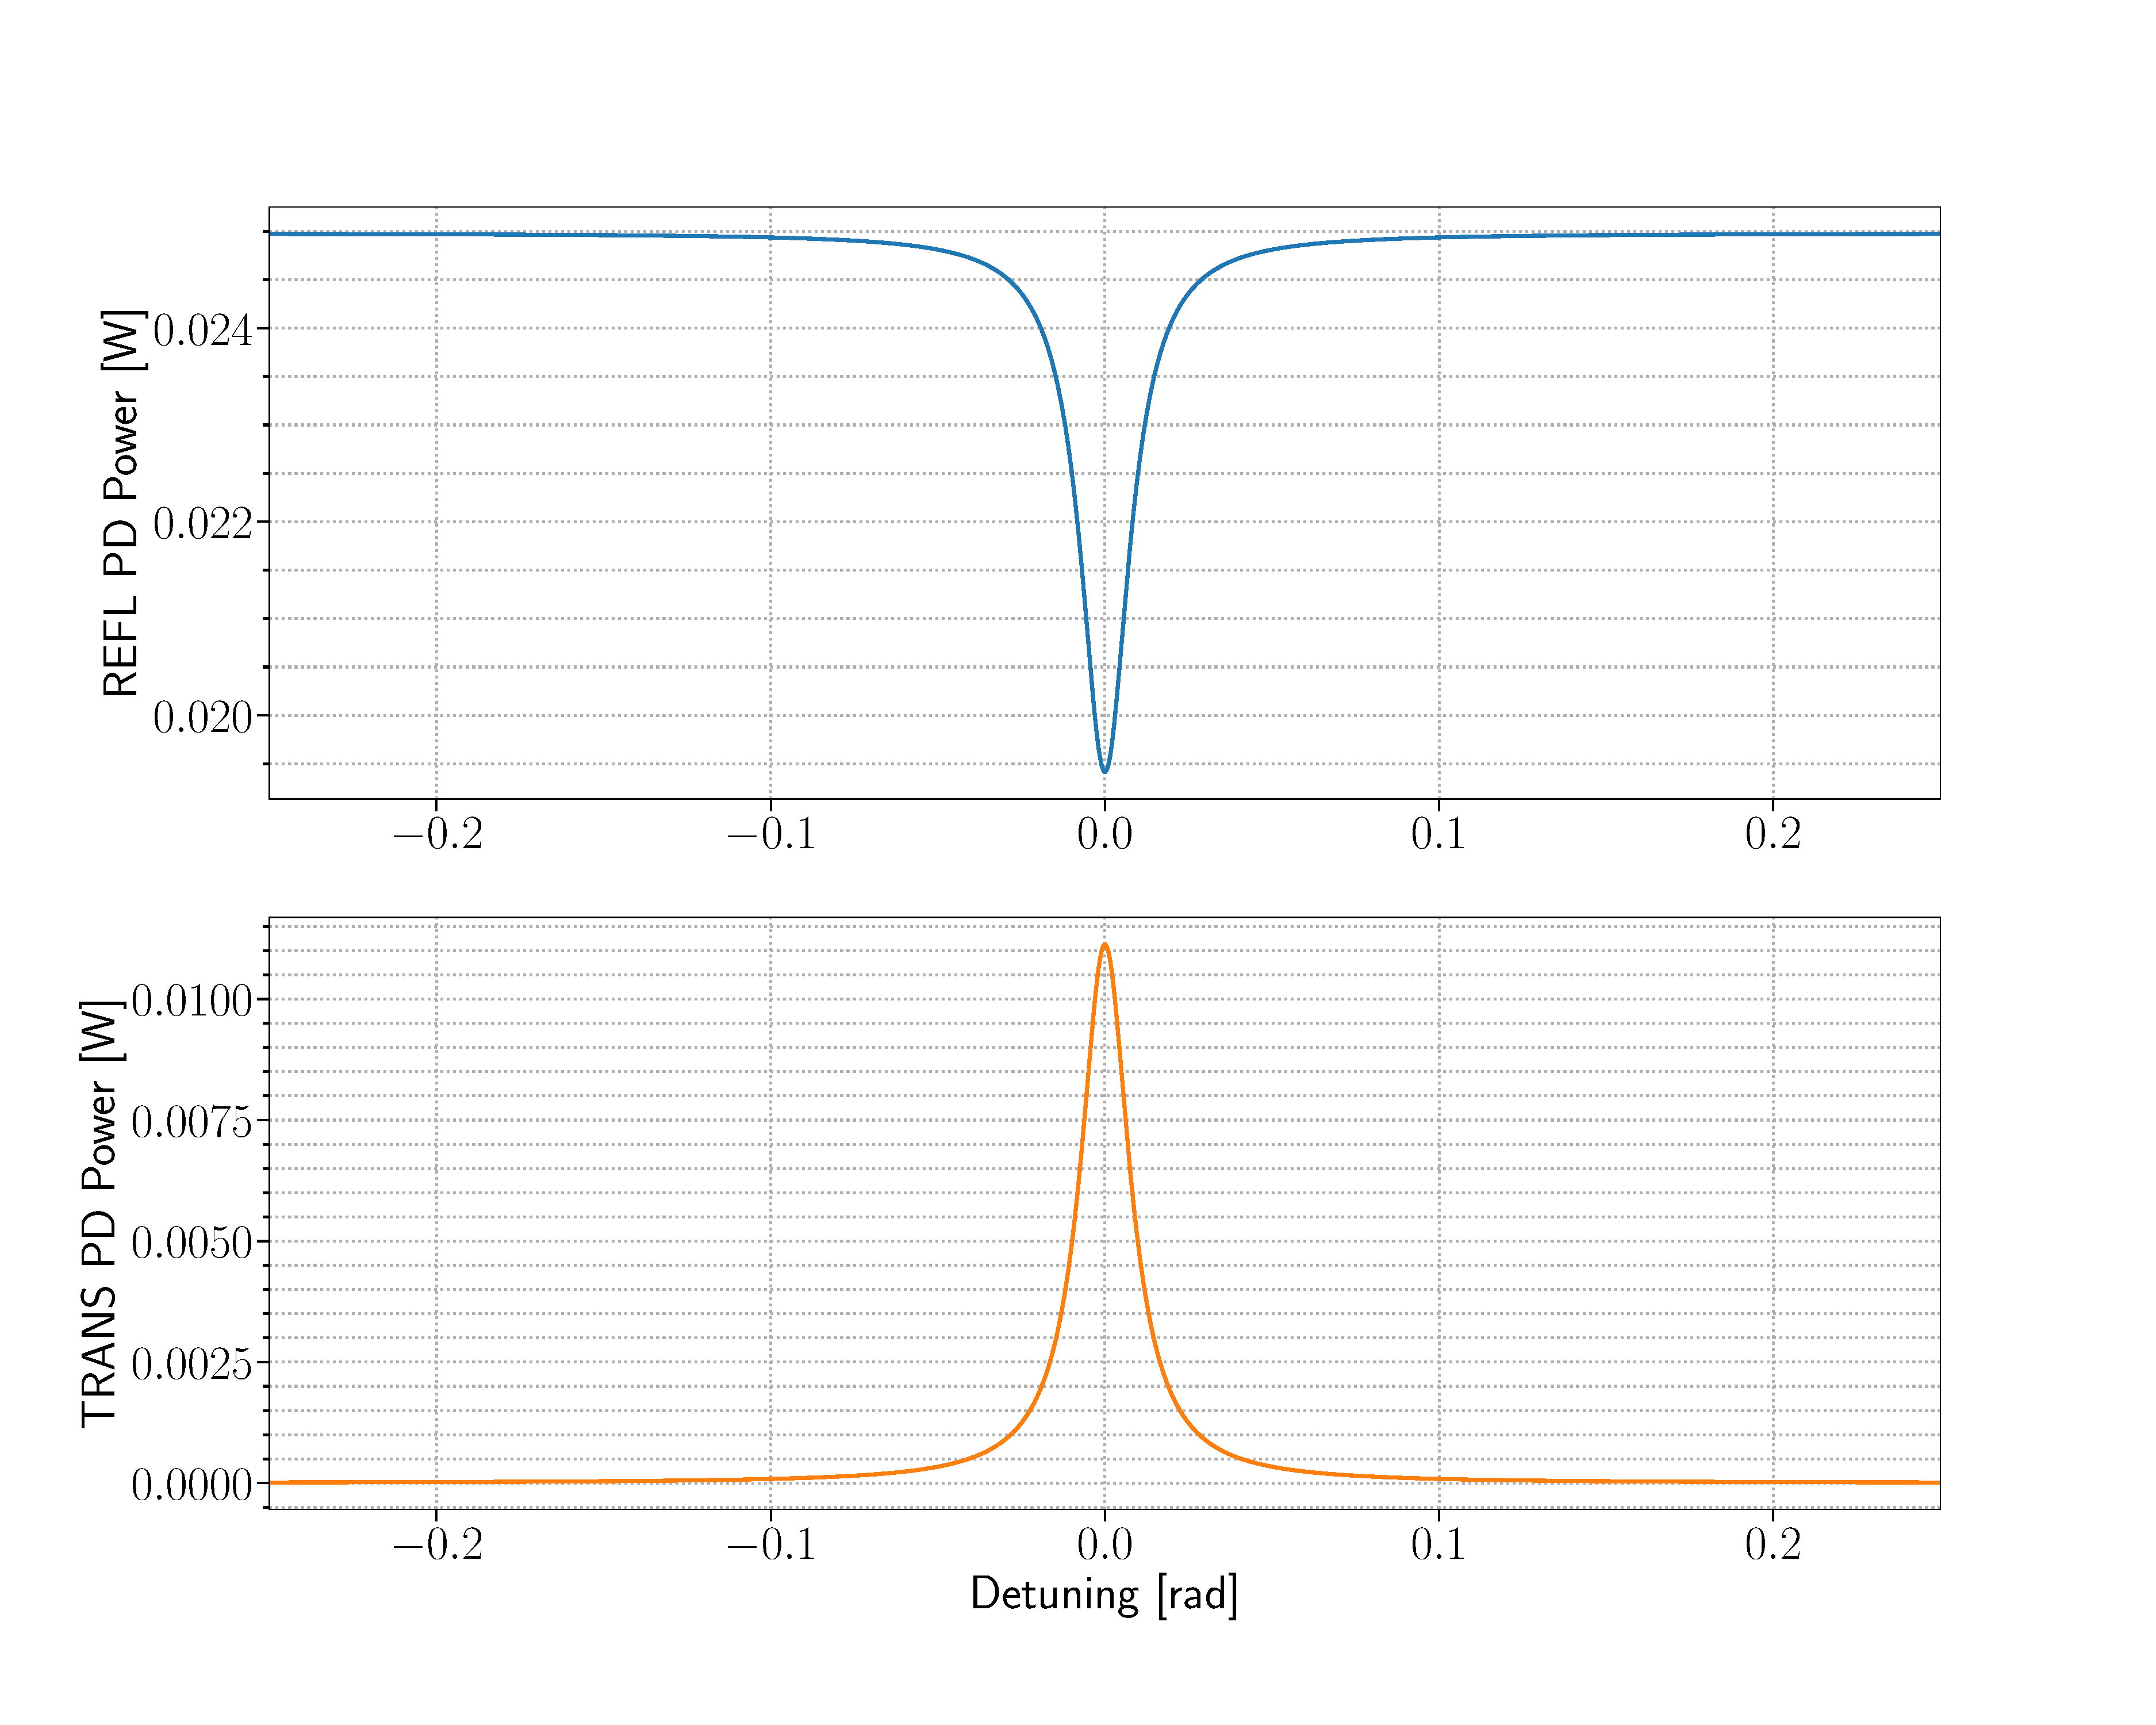
\includegraphics[width=\textwidth]{figs/ALGAAS/DC_power_cav_resonance.pdf}
\caption{Reflected and transmitted power around resonance. \textcolor{red}{Phase as dotted line?}. The resonance peak full width half maximum and the cavity free spectral range can be summarized by a cavity parameter defined as the finessse ($F = \frac{\mathrm{FWHM}_\mathrm{res}}{f_\mathrm{FSR}} = \frac{\pi \sqrt{r_1 r_2}}{1-r_1 r_2}$). The finesse of the cavity used for the figure simulation is ?.}
\label{fig:cav_length_response_DCpow}
\end{figure}

Derived by analogy to the delay line, the Fabry-P\'{e}rot cavity storage time ($\tau_s$) is defined in ~\cite{saulson2017} as:

\begin{equation}
	\tau_s = \frac{L}{c} \frac{r_1r_2}{1-r_1r_2} \approx \frac{L F}{c \pi}
\end{equation}

You may begin to see that the solution for arm elongation is not answered in a literal sense with the Fabry-P\'{e}rot. This is to say that, although there is no physical arm elongation through the usage of Fabry-Perot cavities, a higher sensitivity to differential phase of the light within the cavity for a given cavity length can be achieved and is seen in the difference in the improved frequency response. Though the reader may view the initial part of this discussion of Fabry-Perot cavities as misleading, the intuition gained when addressing their effectiveness for gravitational wave detectors \cite{saulson97}, exhibits the usefulness in this approach.

\begin{figure*}[h!]
  \begin{subfigure}{\includegraphics[width=.45\textwidth,page=3]{INTRO/ifo_configs.pdf}}
  \end{subfigure}
  \hfill
  \begin{subfigure}{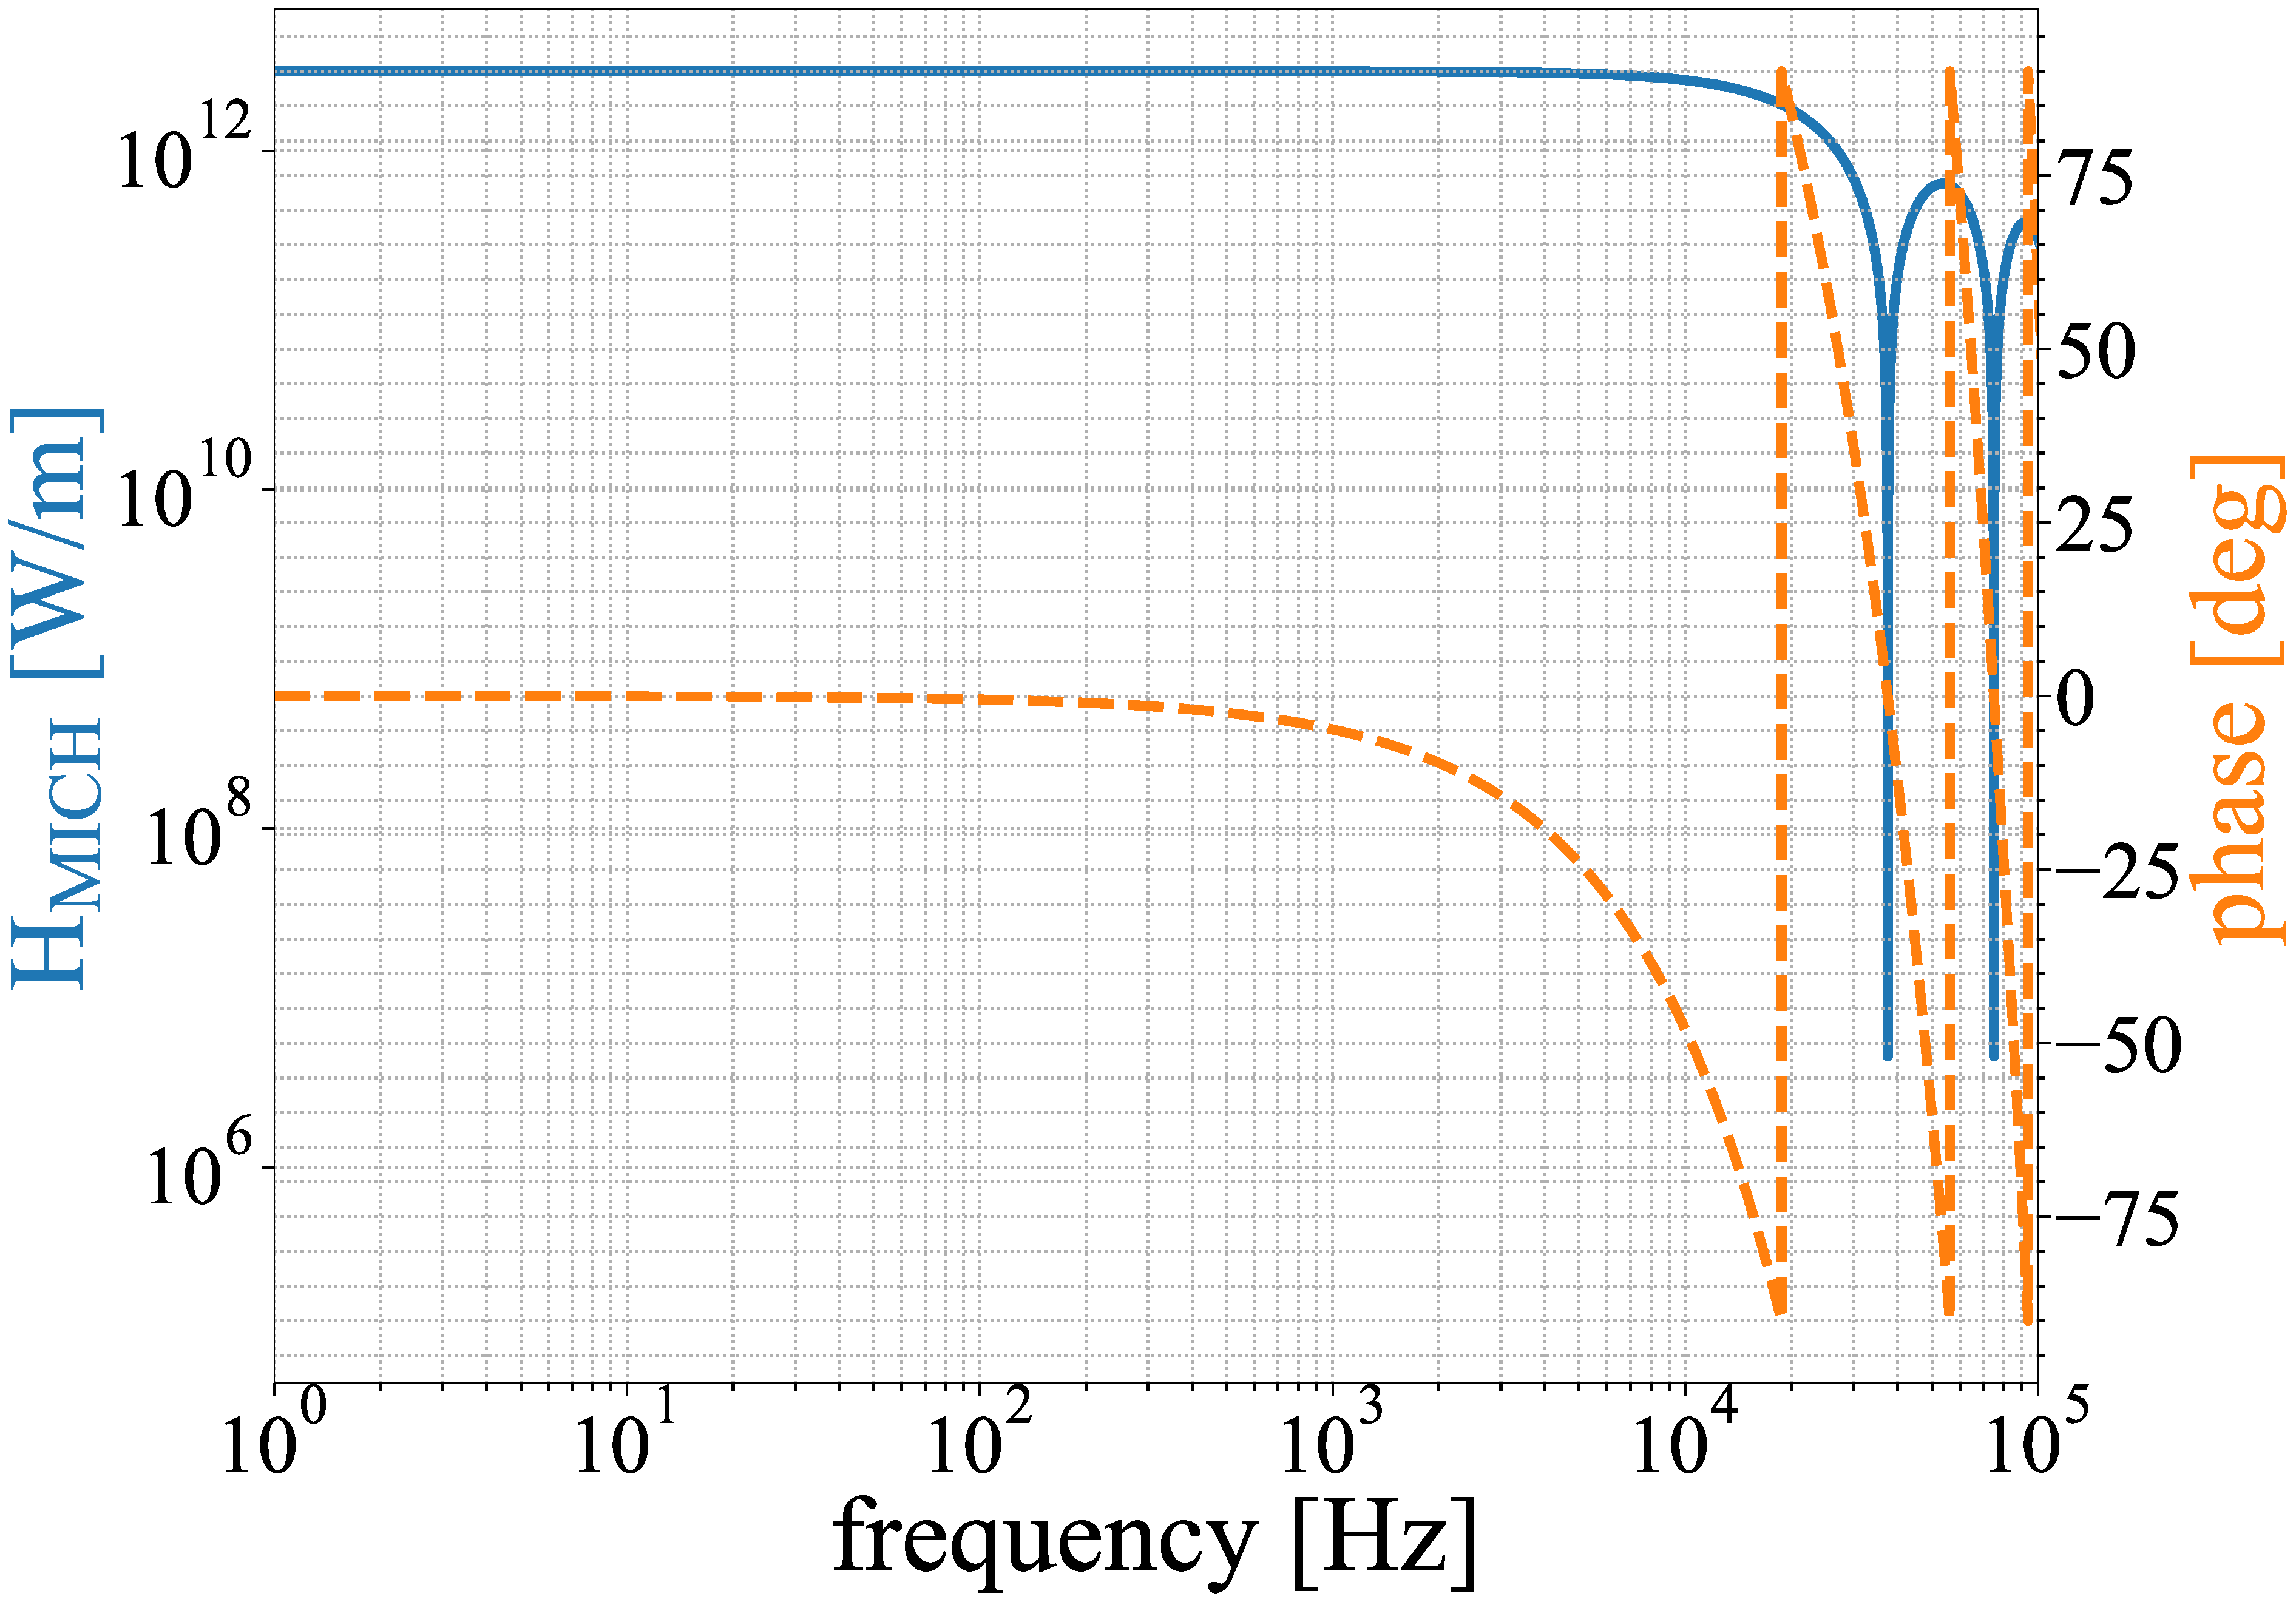
\includegraphics[width=.5\textwidth]{mich_fr.pdf}}%{fpmi_fr.pdf}
  \end{subfigure}
  \hfill
  \caption{\textcolor{red}{PENDING UPDATE} The Fabry-Perot Michelson optical schema with associated differential arm length response (left is optical schema, right is frequency response)}
  \label{fig:fpmi}
\end{figure*}

Advanced LIGO, with it's length and estimated Finesse has a storage time of ?.
It's curious how a laser and two mirrors with empty space between them can be such a ubquitous and invaluable tool in experimental science, though its application for high sensitivity differential phase measurements can provide sufficient explanation for it's use ~\cite{?}. 

\subsection{Dual-Recycled Fabry-Perot Michelson (DRFPMI)}
Recycling mirrors are an extension of the FPMI that provide a means of enhancing the optical gain of the instrument through different means by the nature of their placement at the symmetric and anti-symmetric ports.

\begin{figure}[H]
\begin{center}
\includegraphics[width=\textwidth,page=4]{INTRO/ifo_configs.pdf}
\end{center}
\caption{\textcolor{red}{PENDING UPDATE (also, borrowed figure does not have SR mirror)} The Dual-Recycled Fabry-Perot Michelson optical schema with associated differential arm length response (left is optical schema, right is frequency response)}
\label{fig:drfp_michelson}
\end{figure}


\subsubsection{Power Recycling}
When operating a FPMI, power often gets reflected back to the symmetric port leading to a significant waste of power if simply dumped. An additional partially reflective mirror is placed at said port to recirculate (or ``recycle") that power back to the arm cavities. It's positioning is kept fixed enough so that the input light adds coherently with the laser input, while the macroscopic positioning from ITMX/Y is better understood once addressing optical sidebands.

\subsubsection{Signal Recycling}
This techinique is commonly addressed to last because of it's contribution after considering the response from the PRFPMI. The principle can be understood similarly as most of the prior discussions; the use of a Fabry-Perot as an optical amplifier. By simply placing a mirror at the output port it is understood that you would take whatever light leakage coming from the PRFPMI (caused by differential arm motion) and re-introduce it to the arms. Now the question is, can that light add coherently for a signal that you are interested in detecting? As it turns out, it definitely can but careful choices must be made. Mirror location (macroscopic and microscopic tuning) as well as reflectivity have some interesting impacts to the cavity frequency response. But the general statement can be made: when introducing a mirror of relatively low reflectivity at the anti-symmetric port, you can increase the detector bandwidth but at the cost of reducing the optical gain.


\section{ALIGO}

\begin{figure}[H]
  \begin{center}
	  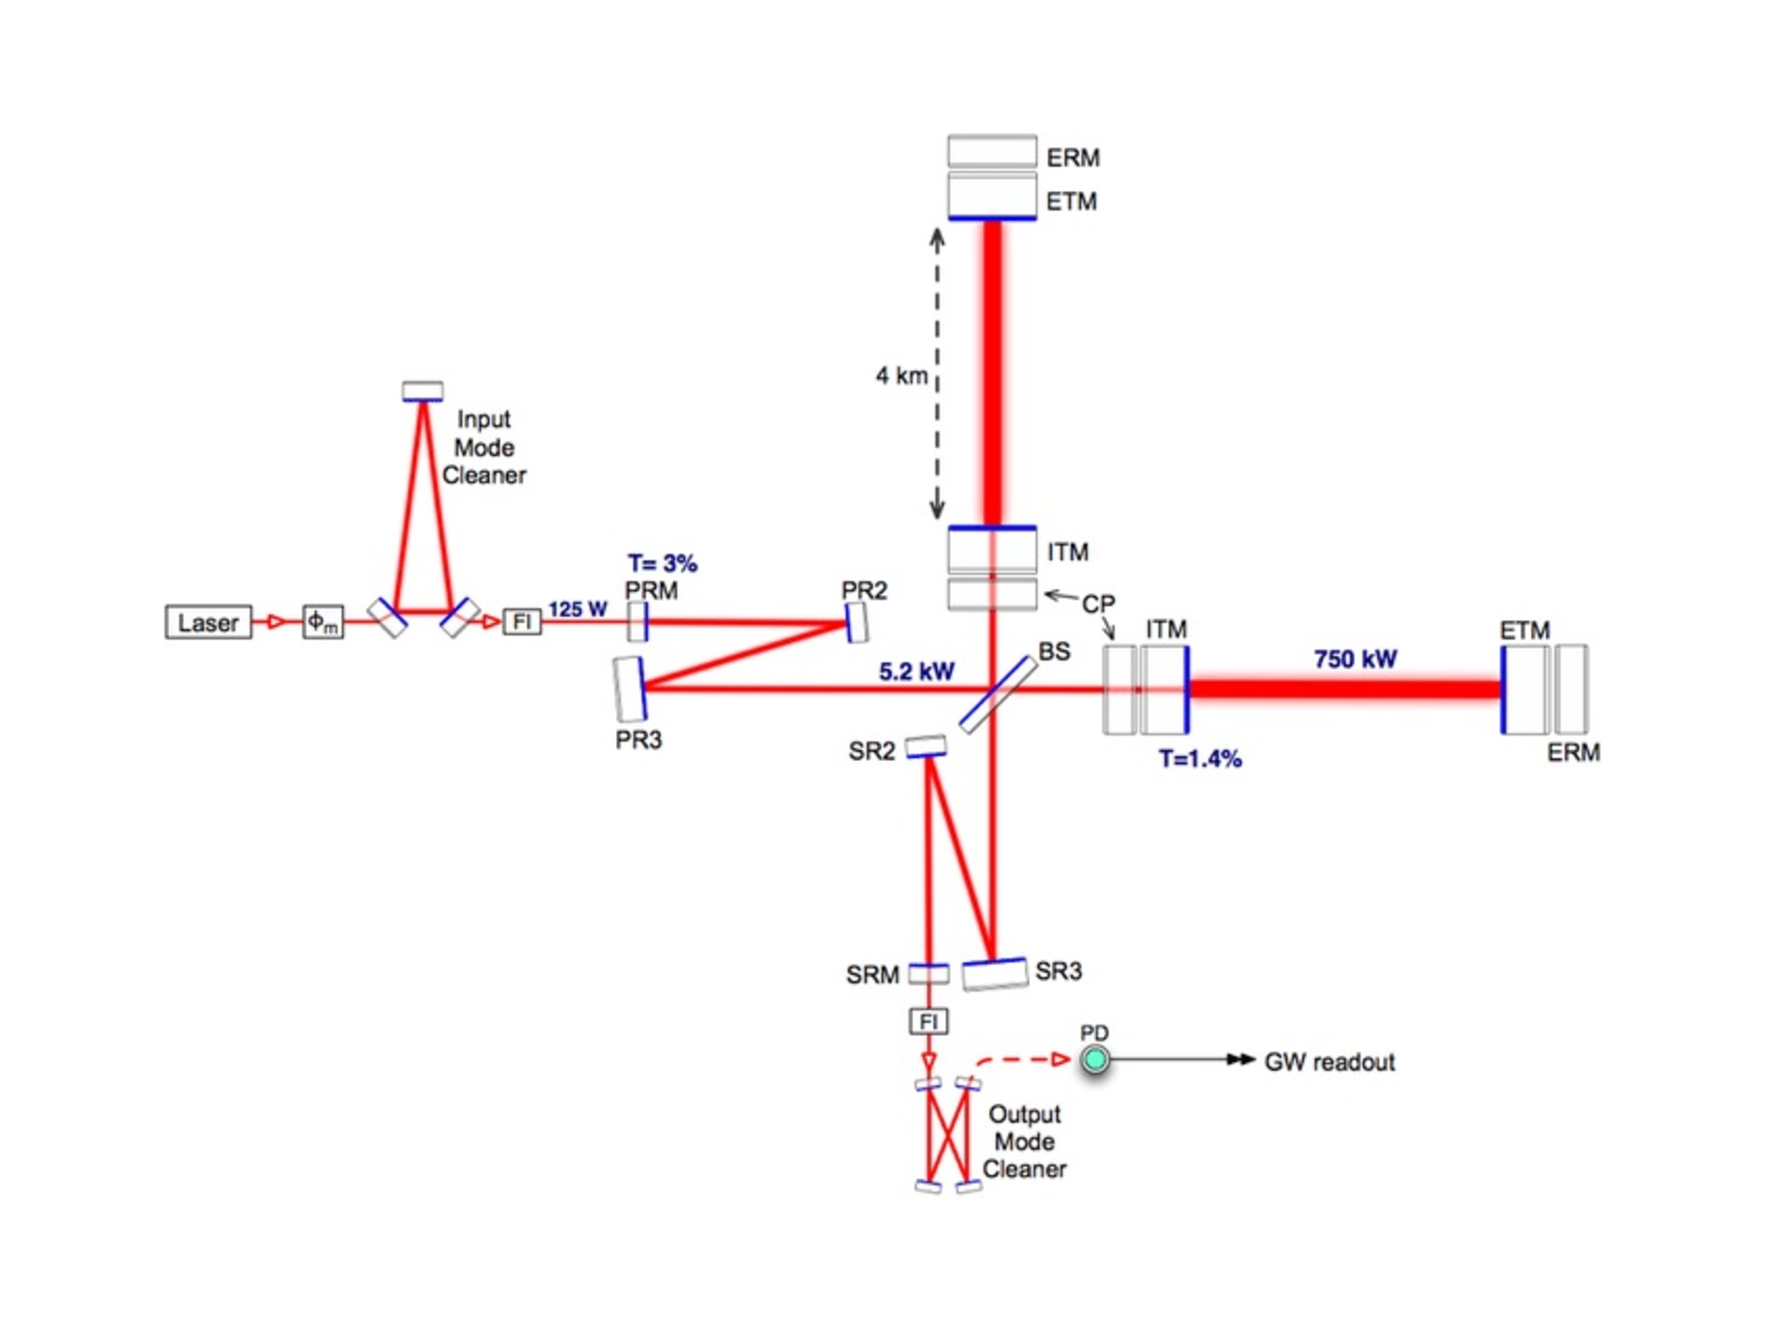
\includegraphics[width=\textwidth]{aligo_config.pdf}
  \end{center}
  \caption{DRFPMI configuration used in ALIGO}
  \label{fig:simple_michelson}
\end{figure}

``Core optics" (Recycling mirrors, Beam splitter, and FP cavity mirrors) are kept suspended with quadruple pendulum suspensions so to decouple seismic activity from the mirror positions.

\subsection{Reaching ``Observing Mode"}
The requirements for the operation of the interferometer require that the interferometer be  ``locked"; meaning that there are some necessary configurations / criteria in order for the instrument to act as an observatory with the designed sensitivity. The objective at hand is to convey to the reader some of the essential interferometer operation criteria as it pertains to this dissertation. Cavity length and alignment stabilization as well as mode matching are some general requirements for observatory operation. The first order requirements of the interferometer with 

\subsubsection{Length Stabilization}
With LIGO's coupled cavity configuration, maintaining mirror positions is imperative. Techniques such as the offset lock (using a DC photodiode to measure the transmitted, reflected, or circulating power within a linear and slightly off resonance point) \cite{} and the Pound-Drever-Hall technique (see \ref{subsubsec:pdh} ) are used to maintain cavity length stabilization. Stabilizing cavity lengths to configure the detector into a highly sensitive differential arm sensor is a process that is worthwhile understanding with more ample discussions ~\cite{Mullavey:12}.

\subsubsection{Gaussian Beams}
So far, we've discussed light and phase fronts in such a manner that hasn't addressed the necessary geometric constraints when using Gaussian laser light. We consider a general complex Gaussian beam mode propogating along the beam axis ($z$) with wavelength $\lambda$.

\begin{equation}\label{eq:gaussian_beam}
E(r) = E_o \frac{\sqrt{[\lambda z_o] / \pi}}{W(z)}e^{-r^2 / W^2(z)} e^{-ikz - ik[r^2 / (2R(z))] + i \zeta}
\end{equation}

Where $E_o$ is a complex amplitude, $r = \sqrt{x^2 + y^2}$ defines the transverse beam coordinates, $k$ is the wave number, $W(z)$ is the beam width, $R(z)$ is the beam radius of curvature, and $\zeta$ is the Gouy phase.

Derived from the paraxial approximation of the Helmholtz equation, this field is not the only solution for optical cavities. Alternative higher order solutions are commonly present and are expressed in terms of two mathematical bases: the Hermite-Gauss and Laguerre-Gauss modes. These higher order modes are more often than not power parasites when operating Fabry-P\'{e}rot cavities as displacement sensors and are a symptom of altered cavity geometry; though by virtue of this they can provide error signals for sensing and actuation schemes. This is what is what is done with ALIGO and is accomplished with the alignment sensing and control (ASC) system and thermal compensation system (TCS) for mode matching actuation.

\textcolor{red}{FIGURE: ALIGO Sensor and Actuation schema?}

\subsubsection{Alignment sensing and control}

\begin{figure}[H]
    \begin{center}
    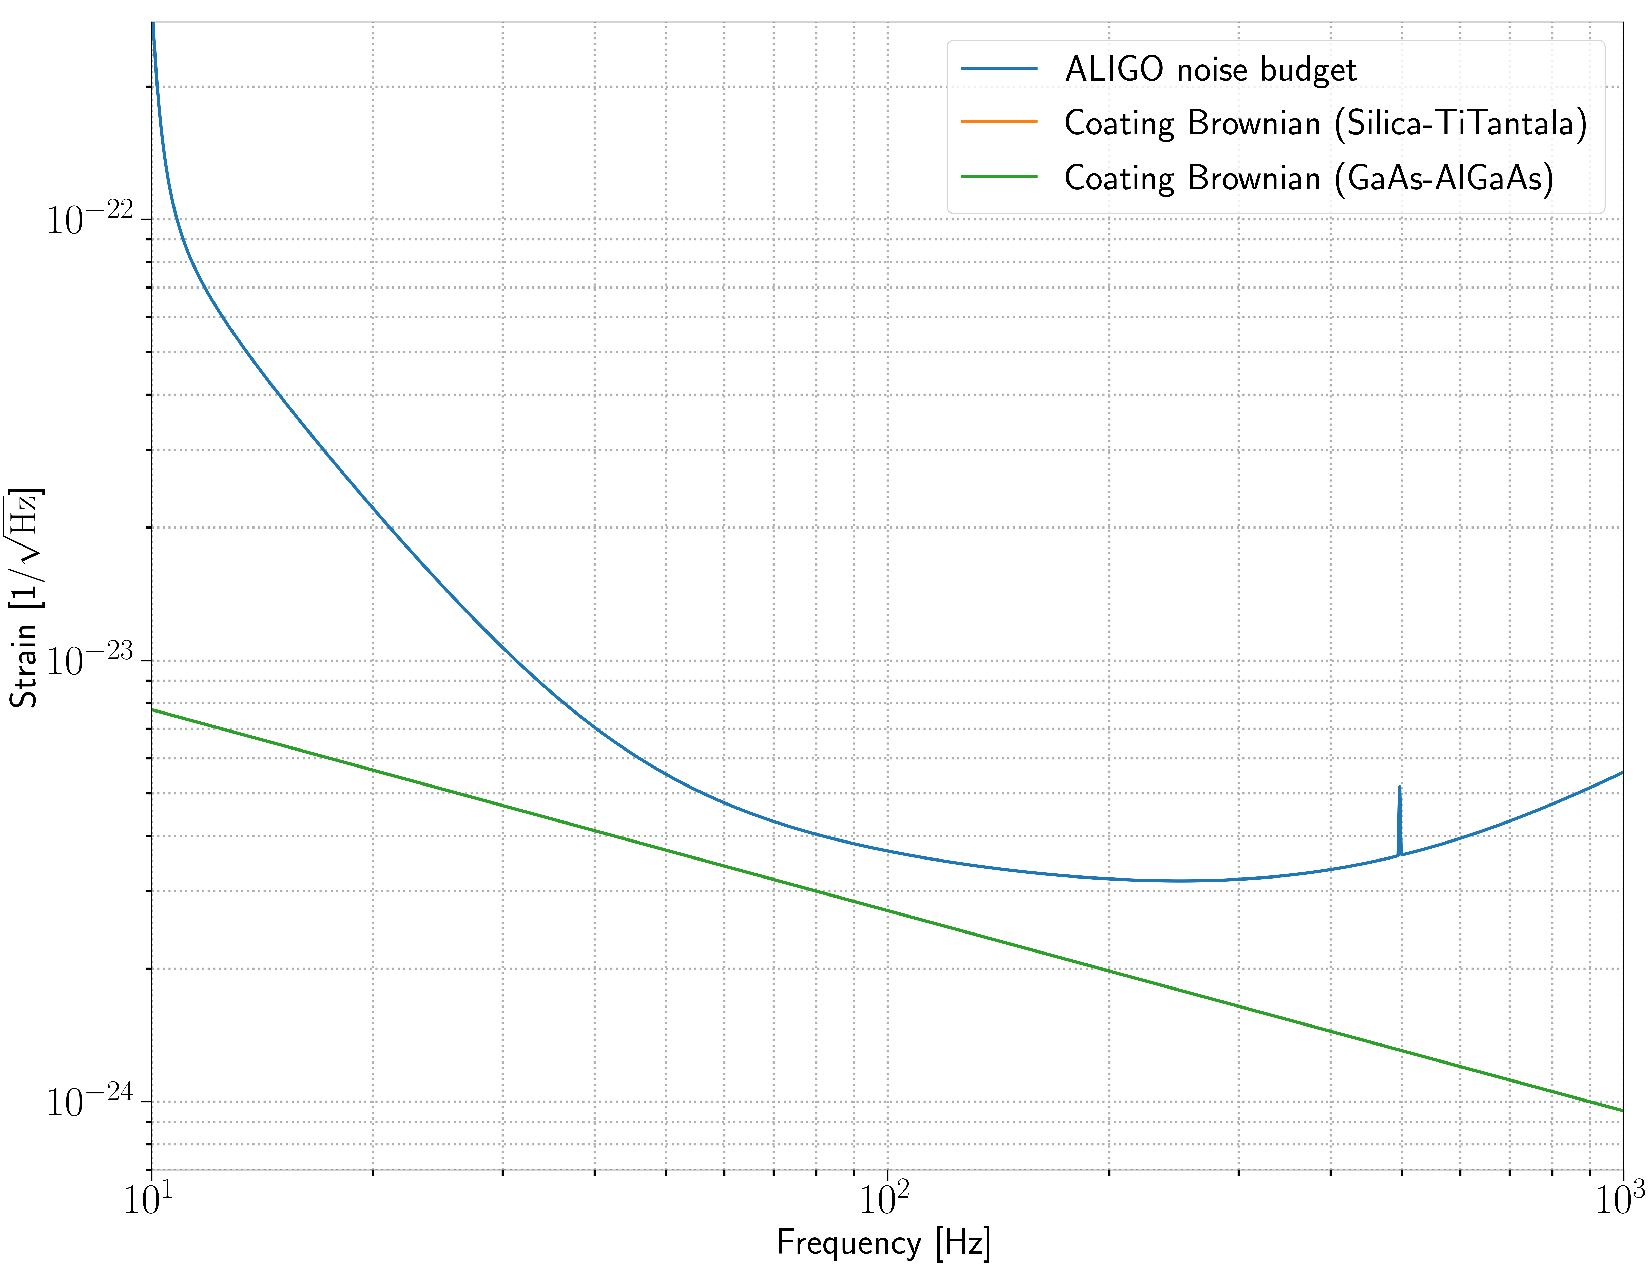
\includegraphics[width=.5\textwidth]{ALGAAS/aligo_nb_plus_cbn.pdf}
    \end{center}
    \caption{A misaligned Fabry-P\'{e}rot cavity scatters circulating light into higher order Hermite-Gauss modes.}
\label{fig:aligo_tn_comparison}
\end{figure}

\begin{equation}
	E_{n,m}(x,y,z) = E_o \bigg[ \frac{W_o}{W(z)} \bigg] H_n \bigg[ \frac{\sqrt{2}x}{W(z)} \bigg] H_m \bigg[ \frac{\sqrt{2}x}{W(z)} \bigg] e^{-(x^2 + y^2)/W(z) - ikz - ik[(x^2 + y^2)/(2R(z))] + i(n + m + 1)\zeta(z)}
\end{equation}

Even with state-of-the-art isolation from ground motion for terrestrial gravitational detectors and high mass mirrors, current gravitational wave detectors still suffer limitations and require sensing and feedback loops to maintain mirror alignments.

\subsubsection{Mode Matching}
For Gaussian beams, there are further requirements of macroscopic mirror positions and radius of curvatures in order to  maximize resonant power in the fundamental mode. Failure to plan and maintain these sucessfully results in a mismatch of the beam mode to the cavity mode and scattering power into higher order Laguerre-Gauss modes.  

\begin{equation}
	E_{n,m}(\rho, \phi, z) =  E_o \bigg[ \frac{W_o}{W(z)} \bigg] H_n \bigg[ \frac{\rho}{W(z)} \bigg]^2 L^n_m \bigg[ \frac{\sqrt{2}\rho^2}{W^2(z)} \bigg] e^{-\rho^2/W(z) - ikz - ik[\rho^2/(2R(z))] - jn \phi + i(n + 2m + 1)\zeta(z)}
\end{equation}

Even with ultra-low absorption fused silica substrates and coatings, circulating power is estimated to reach $\geq$ 200 kW, distorting the radius of curvatures of the arm cavity mirrors by ? m. In LIGO's coupled cavity configuration, these distortions can introduce significant optical loss due to mode mismatch, and as gravitational wave detector sensitivity approaches the quantum noise threshold, we limit ALIGO sensitiviy two-fold with mode mismatch ~\cite{}. The solution implemented in ALIGO to mitigate mode mismatch consists of hartmann wavefront sensors with 800 nm and 833 nm probe beams for providing real-time mirror lensing / surface distortion data, and thermal actuation on mirrors throughout the interferometers with particular focus on the arm cavity mirrors. The thermal actuation of the core optics comes in two types: a CO2 laser actuator impinging upon a pre-installed fused silica compensation plate (CP) for positive lens actuation and an annular ring heater for negative lens actuation \cite{}. 

\begin{figure}[H]
	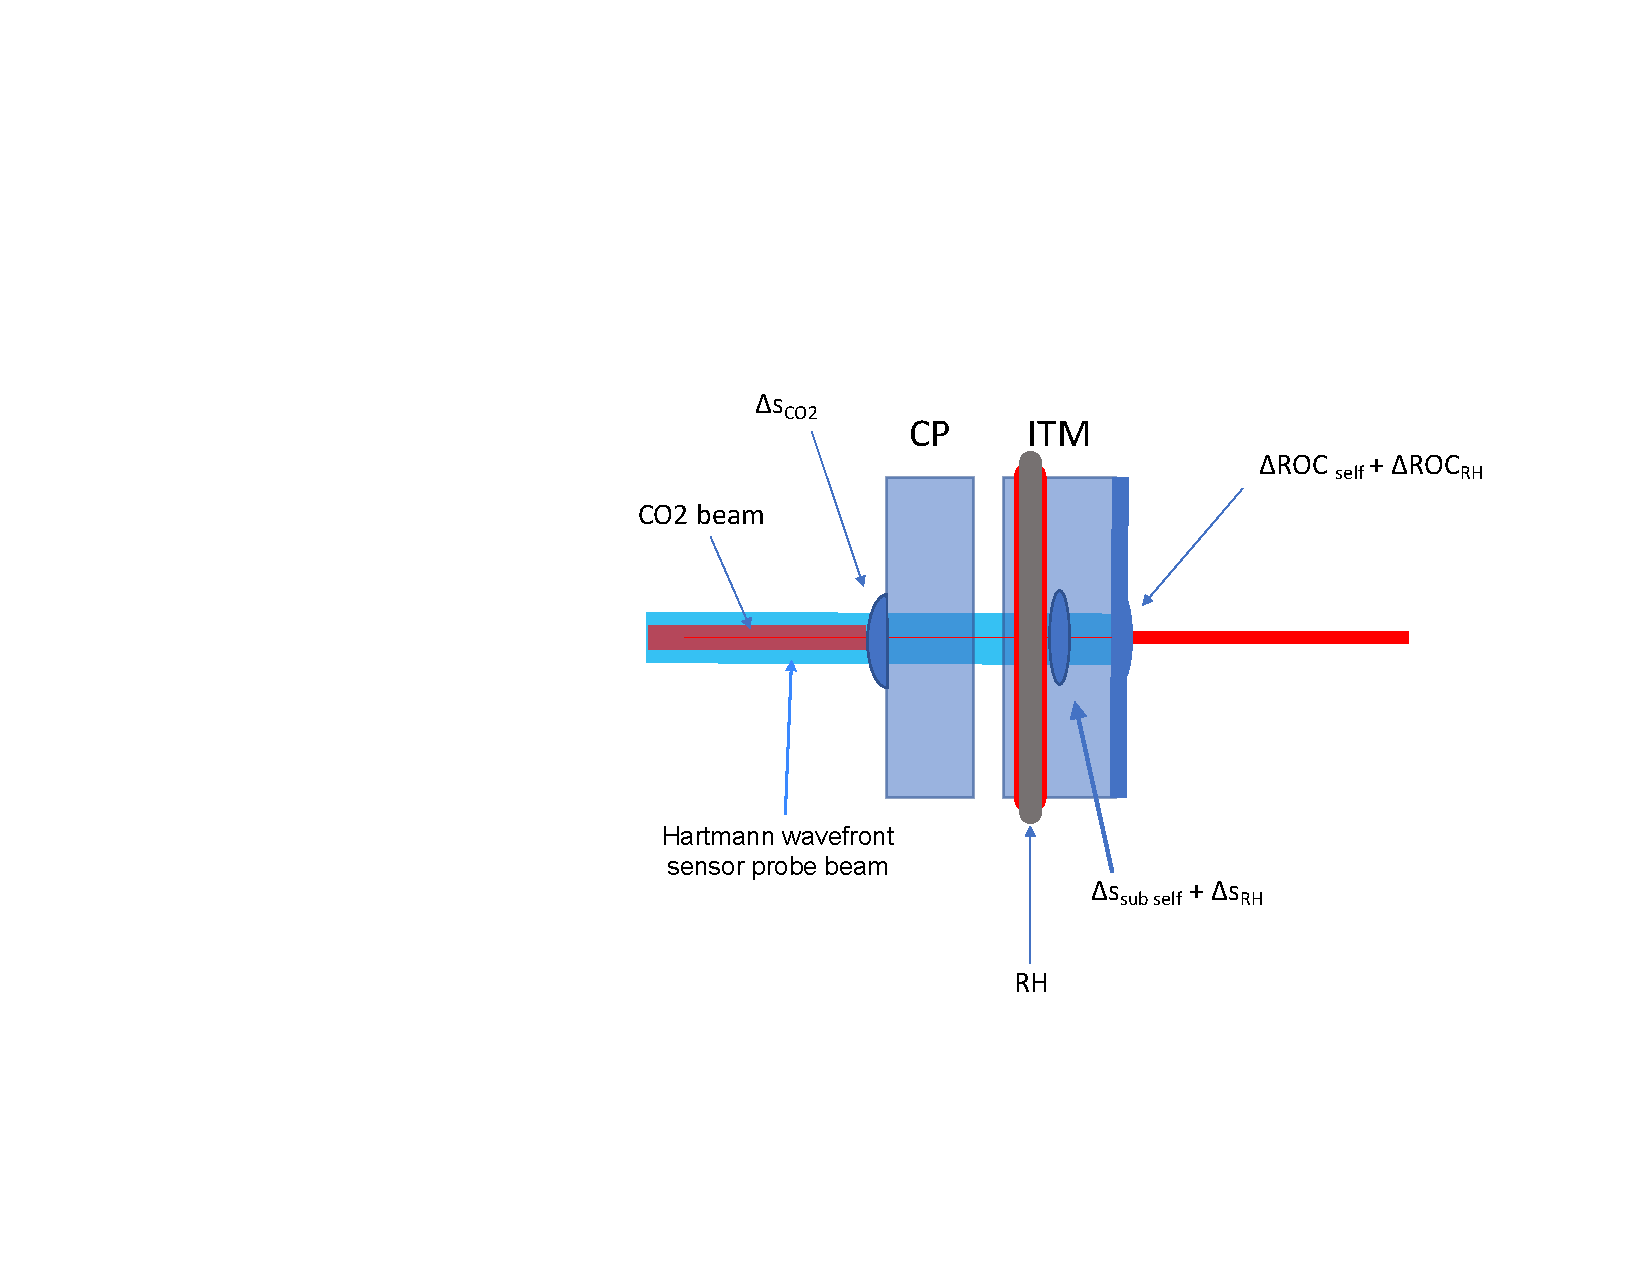
\includegraphics[width=\textwidth]{TCS/FP_input_coupler.pdf}
\caption{Thermal compensation at a single Fabry-P\'{e}rot input mirror coupler for ALIGO.}
 \label{fig:meas}
\end{figure}

\section{Coating Thermal Noise}
Contributions of categorized noises for gravitational wave detectors are organized in a "noise budget", comprised of a collection of technical (noise imposed by the practical operation of the detector) and fundamental (inherent physical limitations of DRFPMIs by design) noise sources that impose limitations on gravitational wave detection.
\textcolor{red}{Contributions of categorized noises for gravitational wave detectors the "noise budget" ((LHO and LLO O3?) or just GWINC?)}

\subsection{Brownian Thermal Noise}
\textcolor{red}{Might move this section back to the $\algaas$ Electro-optic noise chapter}
\\
In 1827 the Scottish botanist Robert Brown noticed a constant motion of pollen particulates on the surface of water; witnessing randomized collisions of the water molecules holding a kinetic energy proportional to the temperature ($k_BT$) \cite{Brown:1828}. It is because of his documented observations we name the phenomena Brownian motion. And although the observations were on motion of particulates in liquids, molecules and atoms within gases and solids also exhibit Brownian motion. For high precision optical experiments operating at room temperature (and higher due to high power resonant beams), understanding how much differential phase noise is imparted on the interferometer light passing through and reflecting from core optics is crucial. This requires knowledge of the mean squared displacement from each degree of freedom of the system which can be realized through the Fluctuation Dissapation theorem. Derived by H.B. Callen and T.A. Welton, the theorem states that for a randomly fluctuating linear force \cite{Callen:1951}:

 %% Further insight into Brownian motion was explored by Einstein where he was able to relate the mean-square displacement of a particle of radius $r_\mathrm{sph}$ on a fluid with viscosity $\eta$.

 %%\begin{equation}
 %%\overline{x^2} = k_B T  \frac{1}{3 \pi \eta  r_\mathrm{sph}}
 %%\end{equation}

 %%This relation has important implications about how the random motion or fluctuations of a particulate (the pollen) is influenced (dissipated) by the viscosity of the surrounding medium (water).

\begin{equation}
F_x^2(f) = 4 k_B T\; \Re[Z]
\end{equation}

 \noindent Where $\Re[Z]$ is the real part of the impedance of the system. This impedance directly relates to equations of motion:

 \begin{equation}
 Z = \frac{F}{\dot{x}}
 \end{equation}

\noindent Another useful form is the power spectrum of the fluctuating motion:
\begin{equation}\label{fdtpsd}
x^2 (f)  = \frac{4k_B T}{(2 \pi f)^2}\; \Re[Y]
\end{equation}

Where $Y$ is the inverse of the impedance or admittance. With this power spectra, modelling and budgeting notable LIGO fundamental noise contributions attributed to the choice of the materials used for mirror substrates, and highly reflective mirror coatings becomes less daunting. Though adequate modelling of internal force couplings for the aforementioned components is required.

\subsubsection{Internal friction in Materials and Loss angle}

Zener provides a model of the internal friction of materials incorporating anelasticity into the equations of motion \cite{zener:1948}:

\begin{equation}
F = k(1+i\phi)x + m\ddot{x}
\end{equation}

Where $m$ is mass attached to a spring with a spring constant $k(1+ i\phi)$ incorporating the degree of anelasticity $\phi$. From equations 3.5 and 3.3 we perform a Laplace transform and acquire the following form of admittance:
\begin{equation}
Y(s) = \frac{\dot{x}(s)}{F(s)} = \frac{-s}{k(1+i\phi) + ms^2}
\end{equation}

\noindent Or more transparently the Fourier representation since we assume a linear time invariant system:

\begin{equation}\label{admitint}
Y(\omega) = \frac{\dot{x}(\omega)}{F(\omega)} = \frac{-i\omega}{k(1+i\phi) - m\omega^2} = \frac{k \omega \phi - i \omega (k - m \omega^2)}{(k-m\omega^2)^2 +k^2 \phi^2}
\end{equation}

\noindent Plugging equation \ref{admitint} back into \ref{fdtpsd}:

\begin{equation}
x^2 (f)  = \frac{2k_B T}{\pi}\frac{k\phi}{(k-4\pi^2 m f^2)^2 + k^2 \phi^2}
\end{equation}
Computing the admittance from a Gaussian beam impinging upon a HR mirror can require expansion of all individual mechanical degrees of freedom of the test mass system across a relevant frequency range, and with that approach convergence is not guaranteed. Saulson and Gonzalez provide an alternative method to computing the admittance coined the ``direct approach" by Levin when computing the noise from a Gaussian beam on a LIGO HR test mass. The admittance can be acquired through:

\begin{equation}\label{admitdirec}
\Re[Y] = \frac{W_\mathrm{diss}}{F_o^2}
\end{equation}

\noindent $W_\mathrm{diss}$ is the dissipated power from the system due to an oscillating force $F_o$. This form of the admittance reveals an important result of the fluctuation dissapation theorem where an undriven system with a dissapative actor, imparts motion to the degrees of freedom via a driving force by virtue of that same actor at finite temperatures. This direct approach also allows the surface pressure applied by the Gaussian beam to interrogate which mechanical modes of the test mass impose a significant energy when \ref{admitdirec} is plugged into \ref{fdtpsd}. In the case of the gaussian beam / uncoated test mass studied by Levin \cite{levin:1998}:

\begin{equation}
S_x(f) = \frac{4 k_B T}{f} \frac{1-\sigma^2}{\pi^3 E_o r_o} I\phi \bigg[1- O\bigg( \frac{r_o}{R} \bigg)\bigg]
\end{equation}

%this requires that the driving force used in a lab mimics that of a force from a centered Gaussian beam.

\textcolor{red}{Refer to Levin appendix for more on how elasticity parameters are introduced?} Where $\phi$ and $E_o$ are the Poisson ratio and Young's modulus respectively, and $O(\frac{r_o}{R})$ contains a correction term contribution as a function of the small beam radius ($r_o$) relative to the mirror radius ($R$).

\subsubsection{Coating Brownian thermal noise}
Further investigations into the beam/optic system utilizing this approach and elasticity theory led to a deeper understanding about Brownian thermal noise contributions from LIGO test masses (substrate, suspensions, HR coating). Levin mentions, with details from Harry, that the noise contributed by a lossy mirror coating is proven to be to be the most significant contributor of brownian thermal noise. Hong provides a power spectral density \cite{Hong:2013}:

\begin{equation}
S_j^X = \frac{4k_B T \lambda \phi_x^j(1- \sigma_j - 2 \sigma_j^2)}{3 \pi^2 f Y_j (1-\sigma_j)^2 \omega_o^2}
\end{equation}

Where X represents bulk and shear with j = odd (material 1) and j = even (material 2) alternating layers representing high and low index materials j = odd (material 1) j = even (material 2) for an HR coating.

\begin{figure}[H]
    \begin{center}
    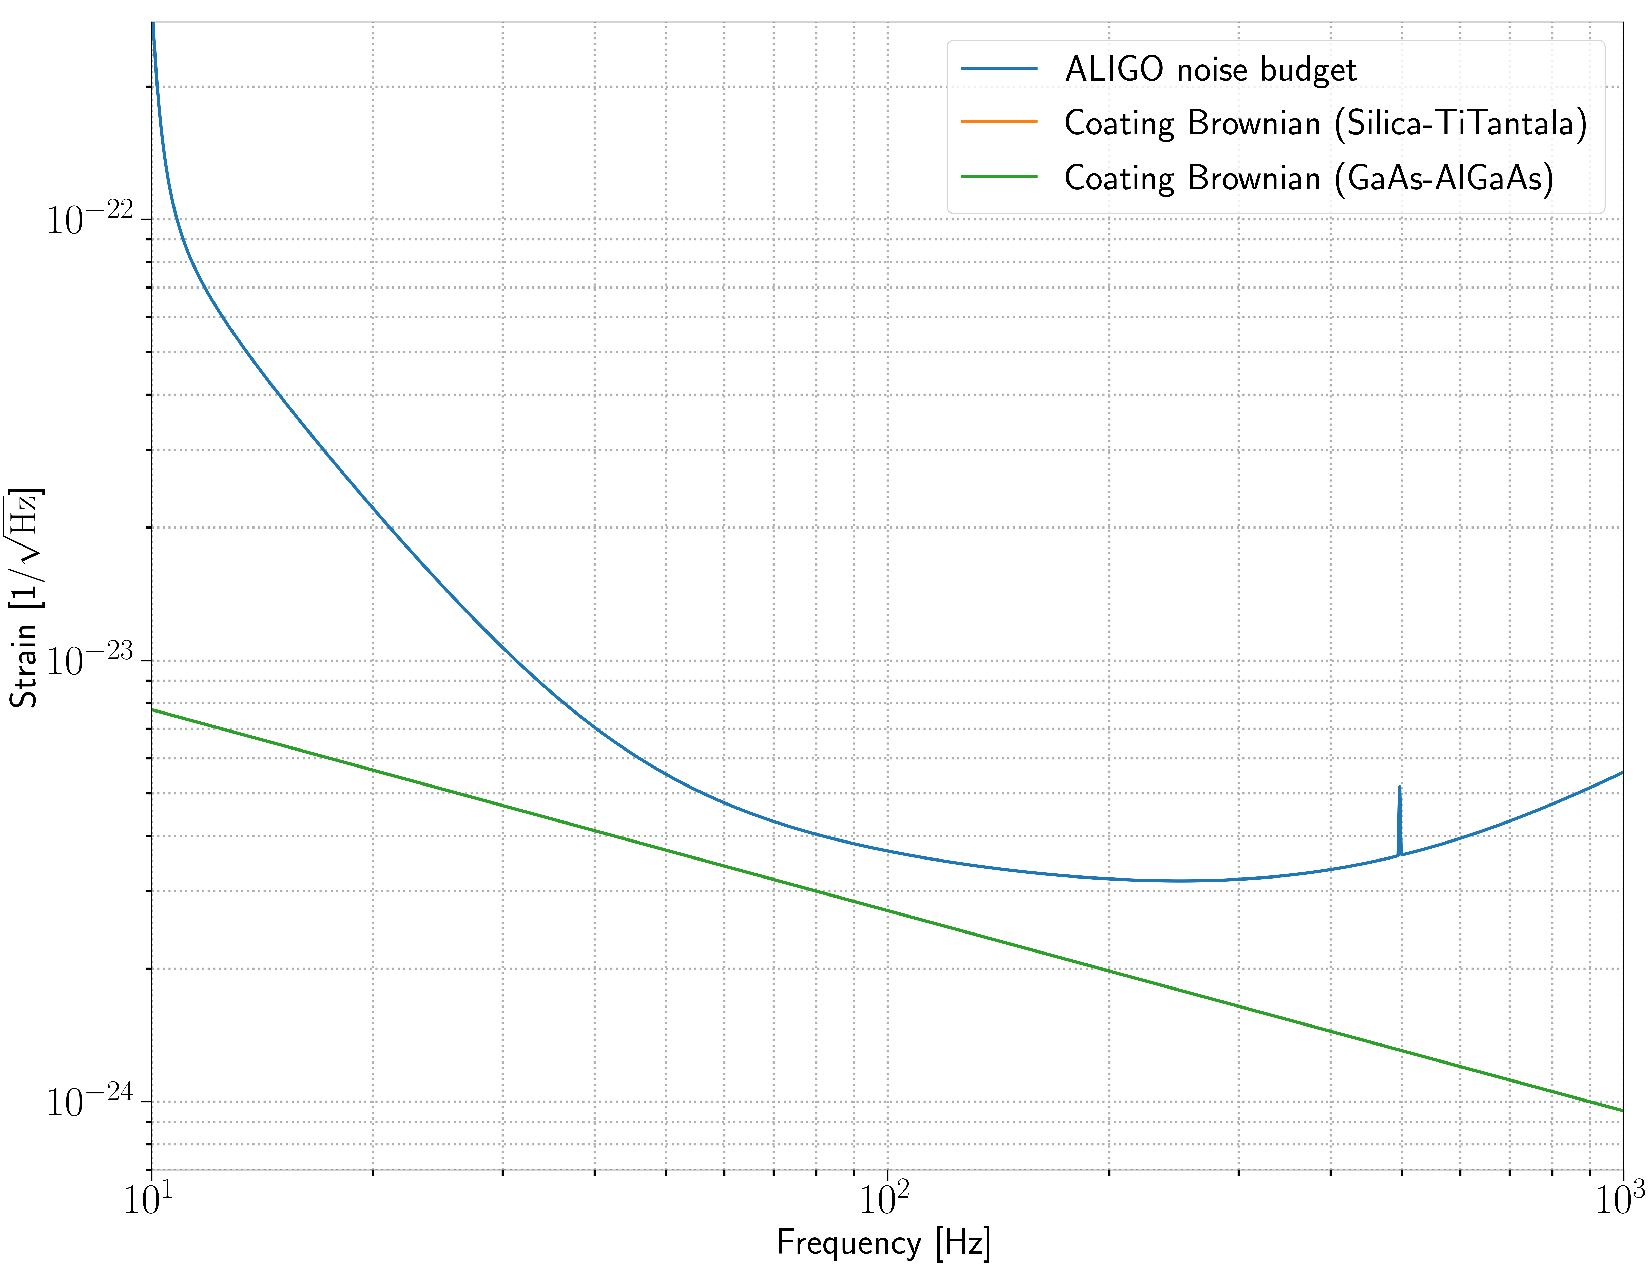
\includegraphics[width=\textwidth]{ALGAAS/aligo_nb_plus_cbn.pdf}
    \end{center}
    \caption{ALIGO noise budget placeholder for silica-tantala, and gaas-algaas brownian noise comparison}
\label{fig:aligo_tn_comparison}
\end{figure}

\subsubsection{$\mathrm{SiO_2}/\mathrm{TiO_2:Ta_2O_5}$ coating parameters}
Currently the LIGO interferometers deposit $\lambda$/4 stacks of silica and titania doped tantala on fused silica test mass substrates. Effective loss angle measurements \cite{Harry:06}

\textbf{Current $\mathrm{SiO_2}/\mathrm{TiO_2:Ta_2O_5}$ elasticity params, power spectra, and strain spectral density (order of magnitude estimate)}

\subsubsection{$\gaas$/$\algaas$ coating parameters}
\textcolor{red}{Specific coating parameters for most promising $\algaas$ candidates? Chat with Steve. Or just mention parameters that are listed in Cole 2013}
\cite{Cole:2013}

\textcolor{red}{Insert computed curves of the most precise and recent (effective) loss angle measurements (Nick Demos measurements?). More instructive to plot strain spectral density or displacement power spectra}

\noindent Currently thermal noise from the $\mathrm{SiO_2}/\mathrm{TiO_2:Ta_2O_5}$ optical coatings is the largest contributor of Brownian noise in LIGO compared to estimated substrate and suspension thermal noise \cite{Harry:06}. As of the end of O3, Brownian thermal noise is estimated to be ? orders of magnitude below the current sensitivity and it will prove to be the limiting source of noise as that sensitivity is increased with various other upgrades mitigating fundamental and technical noise. (\textcolor{red}{already mentioned in intro prior to this thermal noise section. Need to re-iterate in more detail?})
